\subsection{Relevant Technologies}
% compare the available technologies and propose how to apply them to our system

\subsubsection{Sensor Ranging}
% Toby - sensors, haptics basic goal
\noindent Ranging sensors are used to provide distance-to-obstacle information for a plethora of products today. They are popularly found in robotics, where they are able to provide awareness of the surroundings, vehicles, where they enable autonomous navigation, or for smart facility and home solutions, where they detect movement and are used to trigger various actions. FORWARD requires sensors to enable safe navigation and it is thus appropriate to examine the technologies available to determine which to install on the walker. The intent also is two-fold in that it is desired to gain knowledge of what is attainable, namely what information about the surroundings can we provide our processor and how accurate and insightful can that information be. Note that, FORWARD does not implement features of user health status or tracking and so we do not examine GPS as a relevant technology. FORWARD navigates autonomously, and it will do this by use of \textbf{\textit{time-of-flight sensing}}.\\

\noindent \underline{\textit{Ultrasonic}} There are differing variations of ultrasonic sensing technology, mainly varying by their 1) transmitting and receiving hardware, which can be realized as mono or multistatic, 2) emission and detection capability, which stipulates their active or passive status, and 3) their operating frequency \cite{sonar-type}. As far as whether the hardware comes in the form of a multistatic setup or a single transceiver (emits and receives ultrasound), FORWARD's requirements do not necessarily rule out one or the other. Monostatic could be slightly more conducive to mounting on the walker legs and help retain a lower profile because of their smaller (2x) dimensions.\\

\begin{figure}[H]
	\centering
	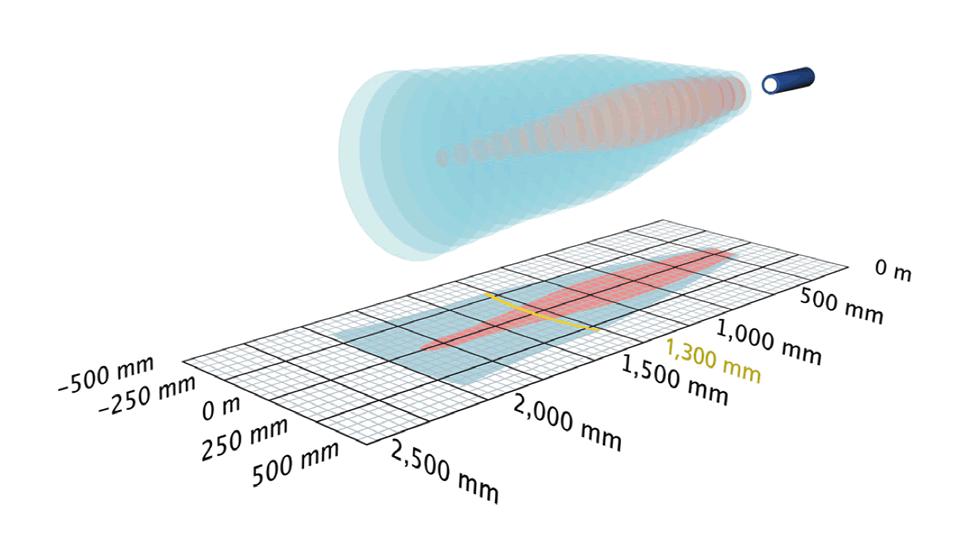
\includegraphics[width=0.7\textwidth]{./Images/cool-ultrasonic-directivity.png}
	\caption{\label{fig:cool-directivity}Ultrasonic Directivity \cite{coolUltraDirect}}
\end{figure}

\noindent \underline{\textit{LiDAR}} We deploy LiDAR in the context of this project as 1) oriented laterally, 2) topographic, and 3) using the scanning method fixed/solid-state (as opposed to swivel or rotating) without flash \cite{lidar-type} (because we are not desiring to create maps). As designers, we must also consider that LiDAR reliability may be affected by the reflectivity of the target objects and ambient lighting of the surroundings. This is one of the primary reasons both sound and light sensing applications are under consideration. Note, figure \ref{fig:lidarazimuth} shows a scanning LiDAR. In this project, the azimuth and elevation difference are both negligible, as the light beam is single-point. Scanning would require another subsystem with servomotors, which is not in specification or budget. By utilizing both sonic and laser sensors however, we can cover a wider range of azimuth. As discussed earlier, the camera is able to cover more elevation for detection.\\

\begin{figure}[H]
	\centering
	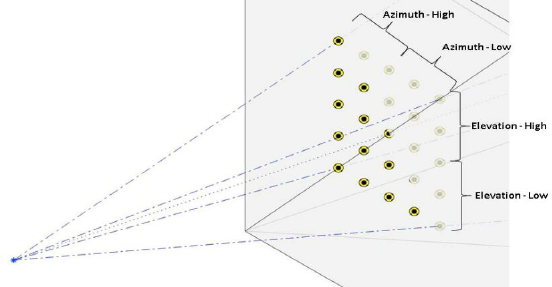
\includegraphics[width=0.7\textwidth]{./Images/FOV-scanning-LIDAR.png}
	\caption{\label{fig:lidarazimuth}Scanning LiDAR FOV \cite{coolLiDARfov}}
\end{figure}

% advanced goal
\subsubsection{Walker Stability} \label{sssec:3_2stability}
\noindent \underline{\textit{Inertial Measurement}} Units are comprised of a magnetometer and accelerometer, which obtain the acceleration and body rate readings of the walker. This is traditionally done by a reading a gyroscope rotation or looking at the magnetic field. It could be greatly beneficial to gain this data, not only for analytical use, but for functionality. Some of the stretch requirements include curb lifting, fall prevention, and incline decline adaptation. With an IMU on-board, the walker can respond appropriately to each scenario. For instance, when lifting over a curve, there can be a certain pitch angle limit imposed to prevent tipover. This is expanded in a similar fashion for fall prevention, where if the user leans too much on the handlebars and causes a tipover, the IMU data can inform the motors of a decision. Finally, the IMU angles are also useful when traversing over inclines or declines. The body rates may also be useful for stability while turning, smoothing the yaw maneuver.\\

\noindent \underline{\textit{Sonar vs. LiDAR for Detection}} As gleaned from \cite{sonar-vs-lidar}, ultrasonic sensors are advantageous for their low cost, simple digital input and output, and wider FOV. However, they lack in their exposure to environment, slower response time, and larger physical size. LiDAR sensors on the other hand, are small and lightweight, and have a fast response time. However, they generally cost more and have a more narrow FOV because of their environmental seal and laser physics.\\

\noindent \underline{\textit{Balanced Sensor Informants}} When comparing the selling points of cameras and traditional sensing methods, we see that each have their advantages. Cameras allow for the most detailed information about the shape and size of the obstacle, but they rely on a lens that can become dirty. The camera may also not operate well in lowlight environments. By still including the ultrasonic and LiDAR, FORWARD can always sense obstacles and have multiple informants. Each sensing method covers the next. When ultrasonic may be affected by wind, the LiDAR is not. When the reflectivity of an object may obscure the LiDAR, the sound waves can still detect. \cite{camera-vs-sensor}.\\

\noindent \underline{\textit{Sensor Fusion}} Implementation of sensor fusion to converge on a most accurate range solution would not be beneficial derived from the ultrasonic and LiDAR outputs, because they should both give nearly identical readings, and thus, leaving no need for fusion. However, it could greatly enhance the computer vision by allowing it to not only identify and classify hazards, but also aid with range detection. The range given by the camera's depth perception could be fused with the more reliable range readings from the front of the walker to further confirm the presence and distance of obstacles. Additionally, the camera could inform the avoidance subsystem of ultrasonic and LiDAR range data to for any reason, ignore.\\

% Matthew - MCU, computer vision, audio
\subsubsection{Computer Vision Object Detection}
\noindent The Object Detection section of our system will be used to identify and alert the user of their surrounding environment. Because of this, we will need our system to be real-time and highly accurate. The main model used for this is known as YOLO. Many of the current object detection applications implement a YOLO model to process the image data. These algorithms works based on the following four steps: Residual blocks, Bounding box regression, Intersection Over Unions or IOU for short, and Non-Maximum Suppression. Residual blocks divide the image into an N by N grid, in which each section becomes a sub-problem. The algorithm then seeks to calculate a resulting vector through bounding box regression. The vector contains the confidence of an objects presence (pc), the image center (bx, by), and the area of the object (bh, bw), resulting in Y = [pc, bx, by, bh, bw, c1, c2]. c1 and c2 are the possible classifications. It's also worth nothing the bh and bw can be greater then the size of the grid. The algorithm then uses intersection over unions and non-maximum suppression to determine what information has the greatest meaning, and thus, we have a prediction. It should also be said that the above describes how to model runs in real time applications, and operates on the assumption that the model has been trained, which in many cases, it has been trained on the MSCOCO data set. \\

\subsubsection{Current Audio Feedback Technologies}
\noindent The Audio Feedback portion of our project needs careful consideration given it's importance in providing the user with audio cues for their environment all the while still being implemented on an embedded MCU, which is likely to contain limited resources. The MCU's considered for this project all contain Bluetooth capabilities and so we will be diving into research for successful products for our application. \\

\noindent \underline{\textit{Bluetooth}} \cite{bluetooth} is another key component to the success of our project. Before looking further into the audio feedback technologies, let us first explain how Bluetooth works and how it will be crucial for our system needs. \\

\noindent To successfully communicate important visual information to our user, we need to do so audibly; and to communicate audibly without interfering with the user with wires. Due to the target users being visually impaired, it is crucial to limit any possible hazards - thus creating a large need for Bluetooth technology. Bluetooth is a wireless communication protocol that transmits on a range centered at 2.45 GHz. Bluetooth is designed to connect clients of short distance, usually 0 to 30 feet, and can be on up to 79 channels. Bluetooth \cite{bluetoothHow} also has two modes: classic and Bluetooth low energy (BLE). Classic is the standard Bluetooth we use daily but BLE is a newer technology which takes classic Bluetooth and makes it low power, which is optimized for close range applications and increased security. Bluetooth protocol allows for it to be very efficient through the concept of \textit{spread-spectrum frequency hopping}. This concept is pictured below in figure 8. \\

\begin{figure}[H]
	\centering
	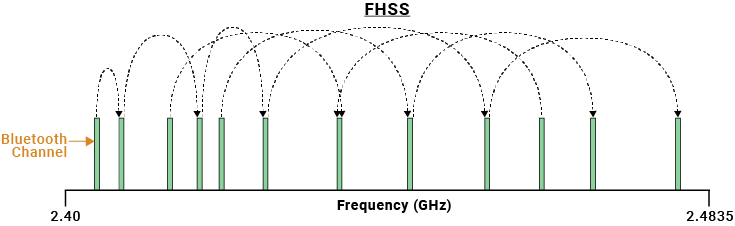
\includegraphics[width=1\textwidth]{./Images/bluetooth-freq-hop.png}
	\caption{\label{fig:bluetooth-freq-hop}Bluetooth Spread-spectrum Frequency Hopping}
\end{figure}

\noindent  Spread-spectrum frequency hopping is when two devices want to communicate, they look for a channel that is available by hopping frequencies. This concept also adds to the security and non-interfering capabilities of Bluetooth because many Bluetooth devices will do this up to thousands of times per second. Bluetooth is mainly used to connect electronics of close ranges, and is commonly used for audio applications - which will be our use as well. \\

\noindent Now, The first technology considered is based upon \underline{\textit{Bone Conduction technology}} \cite{BoneConductionRef}. Bone conduction technology allows users to perceive sound through the vibrations of the bones in the inner ear. One of the main benefits is that audio information can be received even if the ears canals are blocked, which allows for definite communication to the user. Conversely, It also address one of our biggest goals with this system by not obstructing the users ears ways. The bone conduction technology ear pieces sit on the outside of the ear, providing complete freedom for the users ear. Some secondary benefits of bone conduction is increased clarity and reduced background noise as well. While this technology is very advantageous for our goals, some health and comfort disadvantages exist. Prolonged and extraneous use of this technology has been seen to cause hearing loss, vertigo, and tinnitus. This technology can also become uncomfortable to wear for extended periods of time. On average, these headphones have 8 to 12 hours of play time and bluetooth capabilities.  \\

\noindent The second technology considered is \underline{\textit{Ambient Sound Earbuds}}. In order to use a headphone that blocks the ear canal - it would require the use of ambient sound technology to still allow the sound from the outside world. The reason this is of importance is to allow the user to still maintain audible awareness of their immediate surroundings, which if hindered to much, can be severely hazardous. Albeit, even the current state of ambient sound technologies is not the greatest, and can introduce risk for the user having one or two of these earbuds in. The technical  specifications for these product include - 5 to 8 hours of playtime. They cost \$25 to \$50 which can be in our expected range and affordable. \\

\noindent The third technology considered is \underline{\textit{Open Air Bluetooth Speakers}}, coming directly from the chassis on the system. In general, bluetooth speakers are a highly developed technology, which means they are highly reliable with a wide variety of options for our needs. They can cost anywhere from \$20 to \$300, and can run 8 to 20 hours of battery life. The main downside though has public disturbance implications as it would impede on everyone's daily life around the user. The other downside is we introduce risk by not directly relaying the information to the user, such as in a loud room. \\

% Morgan - Power supply, motors, motor shield, steering, braking
\subsubsection{Motor Shield/Driver}
\noindent FORWARD is a system that implements motors to accomplish complex movements, therefore it is required to have a motor driver to interface between the motors and the MCU. Motor drivers are electronic devices that provide the ability to control motors. For example, a DC motor if functional if simply connected to power and ground, however, reversing the direction would take a manual change in polarity and the speed would be constant. Using a motor driver will allow us to control the speed, direction, timing, and torque of the motors \cite{thingbits}. However, these controls do not all occur in one motor driver, but in several varieties of drivers (although can be combined in a motor controller as discussed below). To regulate the power, a motor driver could either use a linear regulator or a switching regulator \cite{etechsparks}. To regulate the speed, there are motor drivers that implement pulse-width modulation (PWM), To control the direction and provide for braking, an H-bridge is used for a motor driver, which uses transistors as switches to change the polarity of the motors. When a positive voltage is applied across the motor, it will operate in the “forward” direction, if a negative voltage is applied to the motor, it will operate in the “reverse” direction, and if the voltage is shorted, the motor will “brake” by coming to a stop \cite{etechsparks}. However, this short-circuiting may cause damage to components in the circuit \cite{coreelectronics}. Another reason why motor drivers are important in general is that the MCU cannot directly control the motors as they are a large load drawing much power \cite{coreelectronics}.\\ 

\noindent Motor drivers are fairly simple devices, while there are also motor controllers, which are devices combining motor drivers that directly connect to an MCU and provide support for a hardware and software interface. Motor controllers typically provide more control than a motor driver because they receive feedback, correct for errors \cite{coreelectronics}, power management and can use several motor drivers all at once, including H-bridge and PWM \cite{powerelectronics}. The motor controller also communicates easily with the MCU using serial communication (SPI, uART, etc.) and often includes libraries that simplify the process of programming the motors. However, motor controllers tend to be more expensive than motor drivers \cite{coreelectronics}. \\

\subsubsection{Speed Control}
\noindent In order to control the speed of the motors, the technology behind this ability is what is known as Pulse Width Modulation (PWM). PWM is a method of allowing the motors to spin for a certain percentage of time within a given a time period. This means that voltage will be applied periodically for a certain duration and will alternate between “on” and “off” For a motor driver set to a duty cycle of 25\%, power is applied to the motor for the first quarter of the period and remains off for the remainder of the period. Because the motor is only operating for a percentage of the time, the motor runs slower than a full duty cycle of 100\%. Meanwhile, a duty cycle of 75\% is a more average velocity between 25\% and 100\%. The figure below illustrates the difference between duty cycles. PWM is the technology used to control the speed of the motors, and is directly set and altered under the software controlling the motors. \cite{etechsparks}. \\

\begin{figure}[H]
	\centering
	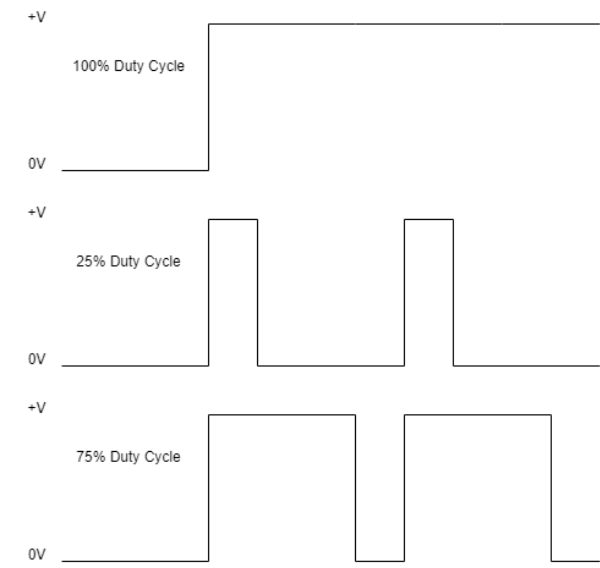
\includegraphics[width=.65\textwidth]{./Images/pwm.png}
	\caption{\label{fig:pwm}Pulse Width Modulation Duty Cycle Graph}
\end{figure}


\subsubsection{Steering and Braking Method }
\noindent One of the main functions of FORWARD is obstacle avoidance, meaning that after sensing and identifying obstacles, the walker must react. In order to dodge obstacles, the walker must steer out of the way of the obstacles, dependent on where the object is detected and the surroundings. One common method of steering, similar to a remote-controlled car, is to use a servo motor to turn an axle containing two of the wheels, at either the front or the back. However, we are using a rollator and not a car. In order to reduce mechanical complexity, as we do not have axles, we will control the steering using individually controlled wheels. Two of the wheels of the walker (either the front two wheels or the rear two wheels) will each have a DC motor. The direction of the product can then be determined by the speed applied to each motor. To illustrate, if the walker detects an object straight ahead and sense that there is an open pathway to the right, it will veer right by keeping the velocity of the left motor constant while decreasing the velocity of the right motor proportional to the angle the walker is turning right. Likewise, if the walker needed to veer left to avoid the oncoming obstacle, the velocity of the left motor will decrease by lowering the duty cycle while the right motor remains at the same velocity.\\ 

\noindent Another aspect to obstacle avoidance is sometimes simply to break. There are instances where it is most beneficial for the walker to come to a complete stop, for example, if the sidewalk ends and leads into the road or if there is no room to pass an obstacle to the left or to the right. In order to accomplish this task, we again wanted to avoid mechanical complexity. A common solution to braking is to use hydraulic brakes that respond to a handle being squeezed. While it is certainly possible to implement hydraulic brakes into our design and automate them mechanically, we desired to exercise our learning in software design rather than mechanics. Thus, our method of applying brakes to our design is to slow down the DC motors driving the walker until the motors turn off and then reverse the direction of the motors until the walker comes to a complete stop. However, there may be a need for locking the wheels, similar to the emergency brake on a car, so that the walker does not roll away from the user when stopped \cite{oxford_health_2014}.\\ 

\subsubsection{Power Supply}
\noindent In order for our FORWARD walker to operate, it needs to have a power source(battery) as well as a power supply to recharge this source. Power supplies are needed to first step down the voltage supplied by an AC source to the needed voltage, then to convert this AC power to DC power, reduce noise of the incoming voltage signal, and finally to regulate the voltage in charging the battery \cite{ActPower}. Since power sources only supply a certain rated voltage, in order to not damage any components, we need to step down our voltage and use a voltage regulator. For example, a 24V rechargeable battery used to power a 21.6V DC motor would need to be stepped down to match the motor at 21.6V, or else the motor could be damaged. The voltage would need to be regulated at this level as well so that the incoming voltage is a steady supply. \\

\noindent We need a battery pack (or multiple) that will be able to deliver enough power both to our motors, our MCU, and other peripherals. It is possible to supply all of these loads with only one battery pack, however, we must take care that the battery pack is suitable to meet the needs of each load. This includes regulating the voltage and current needed per load, accounting for noise (especially from the motors), and using a common ground [45].There is also the option of using a separate power supply per load, which would be much simpler in terms of catering to each specific need of the loads, however, it would be less streamlined and multiple battery packs would need to be recharged or changed. It would be more ideal to have one rechargeable battery pack that we can use to supply multiple loads, each with its own voltage regulation. This will also help to reduce the cost as we will not need to buy a battery for every load. However, since some of our components are very high voltage (12-24V, e.g. motors) and other components are lower voltage (3-5V, e.g. MCU \cite{Espressif1}), we may have two separate power supplies, one for higher voltage components and one for lower voltage components. This is so that we need not drastically step down the voltage and more current/voltage can be supplied directly to the components with larger requirements. As we know from basic circuit theory, a power source supplying multiple loads will need to either divide the voltage (in series) or current (in parallel) between the loads. Thus, it would be beneficial to minimize the number of loads per power supply. Having a separate power supply for the lower voltage components would not be an extra burden of cost to our team since we could use a rechargeable phone battery pack to supply power. \\ 

\noindent When deciding upon a power source, necessary requirements to investigate are the voltage and capacity of the battery \cite{INeedMotors}. When supplying voltage to a load, the voltage supplied must be exact or somewhat lower than the voltage required by the components. This will not be much of an issue as we will regulate the voltage. Since our highest-voltage components are the DC motors driving the wheels, we should not need any voltage source exceeding this voltage. The DC motors decided upon under the parts comparison table have a rated voltage of 21.6V. Loads also draw current from the power source, and in general, the larger current that can be supplied the better. Loads will only draw the current that they are using from the power source, so the rated current requirements of components are minimums, not maximums. Battery capacity is measured in Amp*Hours, meaning that there is a tradeoff between how much current a load can draw and how long the battery is able to supply such current. For example, a battery with 36Ah would be able to provide power to a load drawing 1 amp of current for 36 hours, or it could supply a load drawing 36 amps of current for just one hour. We specified as a constraint in our engineering requirements that FORWARD must be able to go up to 15 miles. Because the average walking speed of the average person is around 3 miles per hour, our product is required to have a battery life of up to 4 hours. Under the parts selection comparison, the motors that we decided to implement are rated to draw 11A of current, so the desired battery capacity needs to be at least 1100mA * 5 hours = 5500mAh. Of course, this is a minimum battery capacity; if the consumer of the product walks slower than 3mph or if the motors draw more current than expected under the data sheet, these factors may prevent the battery from lasting a full 15 miles. \\

\subsubsection{DC Motor Technology}
\noindent Our design for FORWARD involves obstacle avoidance, i.e. using motors to drive, steer, and stop the walker. However, there are many different electric motor technologies to choose from, including DC motors (shunt, series, PMDC, compound, brushless), AC motors (synchronous, induction), and other motors (stepper, servo, etc.) \cite{elprocus1}. We will not be considering the use of stepper and servo motors since they are not designed to rotate 360 degrees \cite{pihut}, which we would need for the wheels to rotate and drive. We will also not be considering AC motors, seeing as they are powered by an AC source \cite{powerelectric} and the FORWARD walker would need to operate with a portable power supply (battery), which supplies DC power. This leaves us with evaluating the different types of DC motors. DC motors operate with 3 basic parts: the stator, rotor, and commutator \cite{elprocus2}. The stator is a stationary part that produces the magnetic field that rotates the rotor, while the commutator allows the motor to continue rotating. \\

\noindent \underline{\textit{Shunt DC}} motors are DC motors that include the DC power supply, shunt field, and armature all in parallel. Shunt motors are known for their ability to regulate their speed easily, and they can also increase in speed without the typical drawback of reducing torque by increasing current. These motors are most commonly used where a constant speed is desired, for example, a machine in an assembly line or a fan \cite{elprocus3}. \\

\noindent \underline{\textit{Series DC}} motors are DC motors that include the DC power supply, shunt field, and armature all in series rather than parallel. Because the circuit is one loop, each of these components use the same current and the current is not divided between components. This allows for a very strong magnetic field and thus a strong starting torque with a simple design. However, the series motor does not allow for very good speed regulation and there is a large tradeoff between speed and torque \cite{elprocus4}. \\

\noindent \underline{\textit{PMDC (Permanent Magnet DC)}} motors use a permanent magnet in order to generate the magnetic field. The circuit is very similar to a series DC motor, except the circuit components are the voltage supply, back emf, and armature resistance. PMDC motors are generally smaller and cheaper than other DC motors because they do not need windings, however, there is a capacity to the flux generated by these motors. These motors are most applicable where a smaller motor is needed, such as kitchen appliances and windshield wipers \cite{elprocus5}. \\

\noindent \underline{\textit{Compound motors}} combine shunt and series DC motors into one technology. The circuit combines the DC source in series with the shunt field and armature combined in parallel. This allows for the series advantage of a larger starting torque and the shunt advantage of good speed control. These motors are typically used in applications where a larder load is being driven, such as elevators \cite{linquip}. \\

\noindent \underline{\textit{Brushless DC (BLDC)}} motors are DC motors that use an electronic commutator to continue the motion of the motor rather than a physical commutator and brushes. The electronic commutator switches the voltage of the motor as the rotor rotates to a certain position so that the motor can rotate a full 360 degrees. BLDCs also use a permanent magnet that rotates along with the rotor that creates a magnetic field and is driven by the current. These motors are compatible to be controlled by microcontrollers, efficient, have minimal noise, and have high longevity, therefore they are used in a wide variety of applications, from transportation to everyday devices \cite{elprocus6}. The main drawback to BLDC motors is that they tend to be less cost-effective than brushed motors because they are newer to manufacturing and use electronics \cite{monolithicpower}. Brushless DC motors therefore are much higher quality of motors, however, they will need to be compared with brushed DC motors to determine if there are motors of comparable price. \\

\noindent Power and speed will be necessary considerations as well in deciding which motors we need, as well as what we can afford in our budget. Given our constraints, the walker can weigh up to 60 lbs., plus the weight of the person leaning against the rollator can be up to 37\% \cite{lee2019} their body weight (rollators are typically rated for ~330lbs. \cite{trionic}) and the wheels can be as small as 6”. To achieve speeds of up to 6mph, the motors need to provide at least 336 rpm \cite{spikevm} Using a calculator, we found that for a 60lb electric bike, 122.1lb (37\% * 330lbs) rider load, and a frontal area of $6.72ft^2$ (area of the walker plus the area of the person above the walker \cite{drive}\cite{xconvert}) we would need 267W of power to achieve 6.0mph \cite{gribble}. This calculator takes into consideration the effects of friction, air resistance, and the percent gradient for a hill. While a walker is not exactly the same as an electric bike, they both carry a rider and need to achieve a certain speed. The main differences between a bike and a walker are that a bike bears the full body weight of a person and bikes have much larger wheels than the walker. However, we already calculated the rider load to only be the percentage of the body weight that is bore by the walker, and smaller wheels actually require less power \cite{oxwheels}, providing a buffer so that it is possible the walker will need less than 267W of power. However, since we are using 2 motors, we can use 2 150W motors, which should add up to 300W of power \cite{ebikesforum}. \\